\section{概念设计}

\subsection{实体和属性}

\subsubsection{用户 (User)}

用户实体存储了系统用户的基本信息,包括用户标识、用户名、密码、邮箱、联系方式和用户类型。主键是用户标识,用于唯一标识每个用户。如\cref{fig:entity-user}所示,具体介绍如下:

UserID:用户标识,主键。每个用户的唯一标识符,用于区分不同的用户。
Username:用户名,用户在系统中的登录名。每个用户名在系统中必须是唯一的。
Password:密码,用户登录系统时使用的秘密信息。系统应对密码进行加密存储,确保用户账户的安全性。
Email:邮箱,用户的电子邮件地址。用于系统通知、密码找回等功能,每个邮箱在系统中必须是唯一的。
Contact:联系方式,用户的联系电话或其他联系方式。用于在必要时联系用户。
UserType:用户类型,用于区分用户的角色,如普通用户、警察、管理员等。根据用户类型,可以赋予不同的权限和功能。

\begin{figure}[htbp]
    \centering
    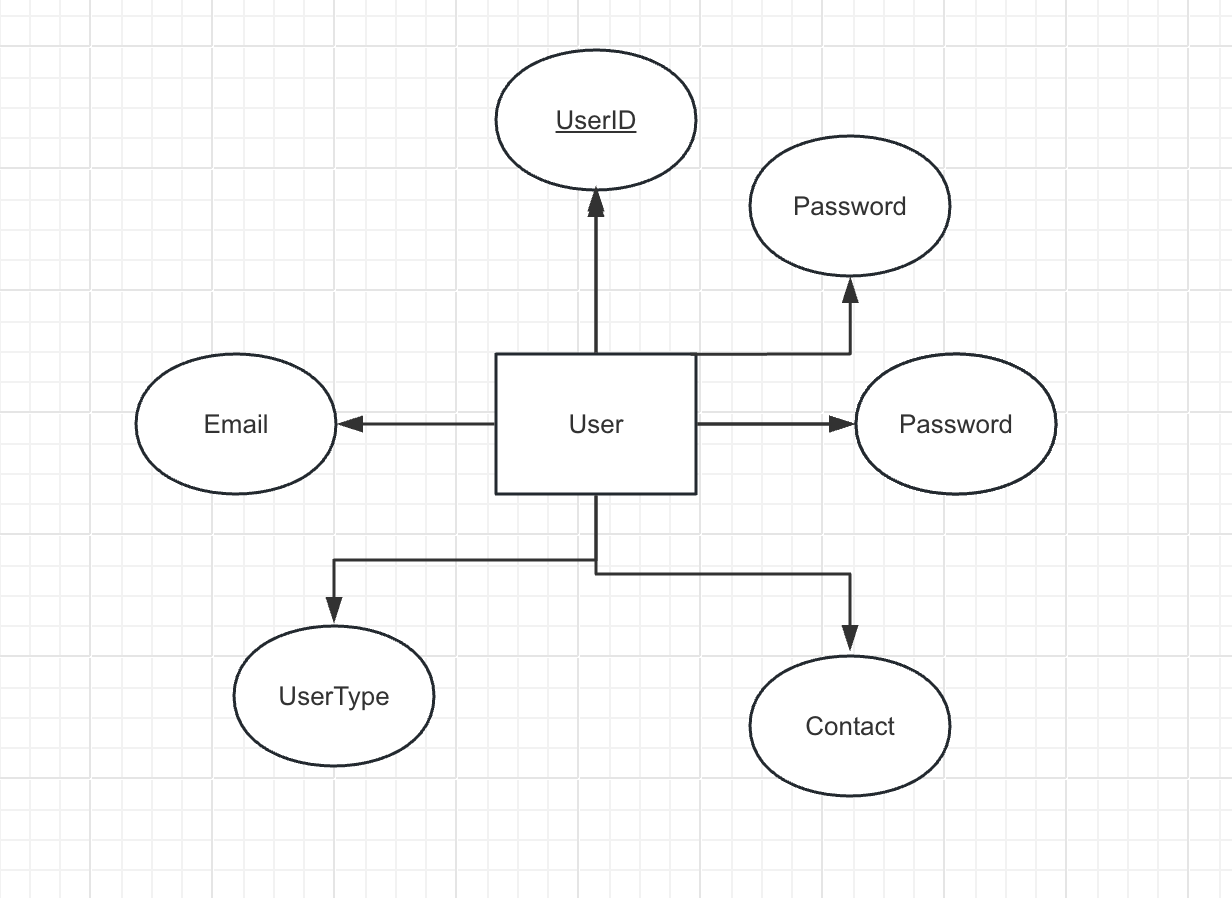
\includegraphics[width=0.5\textwidth]{figures/db-img-01.png}
    \caption{用户实体图}
    \label{fig:entity-user}
\end{figure}

\subsubsection{事件 (Event)}

事件实体存储了系统中所有犯罪事件的详细信息,包括事件标识、事件类型、事件描述、发生时间、发生地点、上报用户ID和审核状态。主键是事件标识,外键是上报用户ID。如\cref{fig:entity-event}所示,具体介绍如下:

EventID:事件标识,主键。每个事件的唯一标识符,用于区分不同的事件。
EventType:事件类型,描述事件的类别,如盗窃、抢劫、袭击等。用于分类和统计不同类型的事件。
Description:事件描述,详细描述事件的经过和相关信息。提供足够的信息以便处理和分析事件。
EventTime:发生时间,事件发生的具体时间。用于记录事件的时间维度。
Location:发生地点,事件发生的具体位置。用于记录事件的空间维度。
ReporterID:上报用户ID,外键,引用用户实体中的UserID。用于标识事件的上报者。
Status:审核状态,描述事件的处理状态,如未处理、处理中、已处理等。用于跟踪事件的处理进度。

\begin{figure}[htbp]
    \centering
    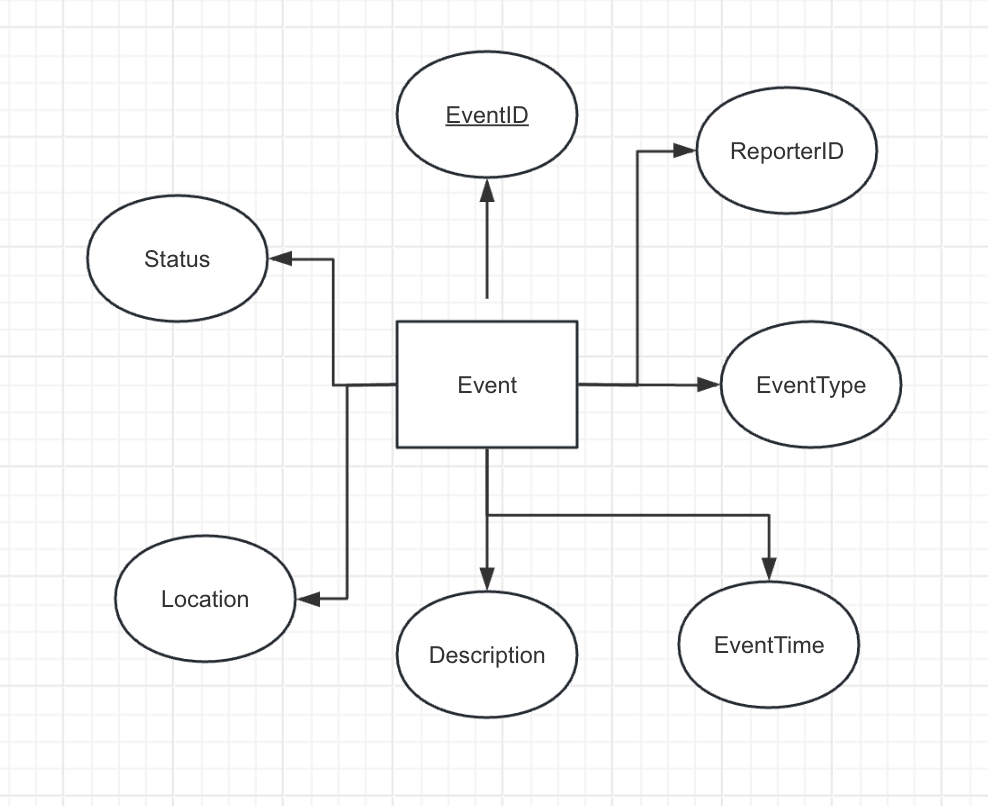
\includegraphics[width=0.5\textwidth]{figures/db-img-02.png}
    \caption{事件实体图}
    \label{fig:entity-event}
\end{figure}

\subsubsection{多媒体文件 (MediaFile)}

多媒体文件实体存储了与犯罪事件相关的文件信息,包括文件标识、事件ID、文件路径和文件类型。主键是文件标识,外键是事件ID。如\cref{fig:entity-mediafile}所示,具体介绍如下:

FileID:文件标识,主键。每个文件的唯一标识符,用于区分不同的文件。
EventID:事件ID,外键,引用事件实体中的EventID。用于标识文件所属的事件。
FilePath:文件路径,文件在系统中的存储路径。用于定位和访问文件。
FileType:文件类型,描述文件的类型,如图片、视频、音频等。用于分类和处理不同类型的文件。

\begin{figure}[htbp]
    \centering
    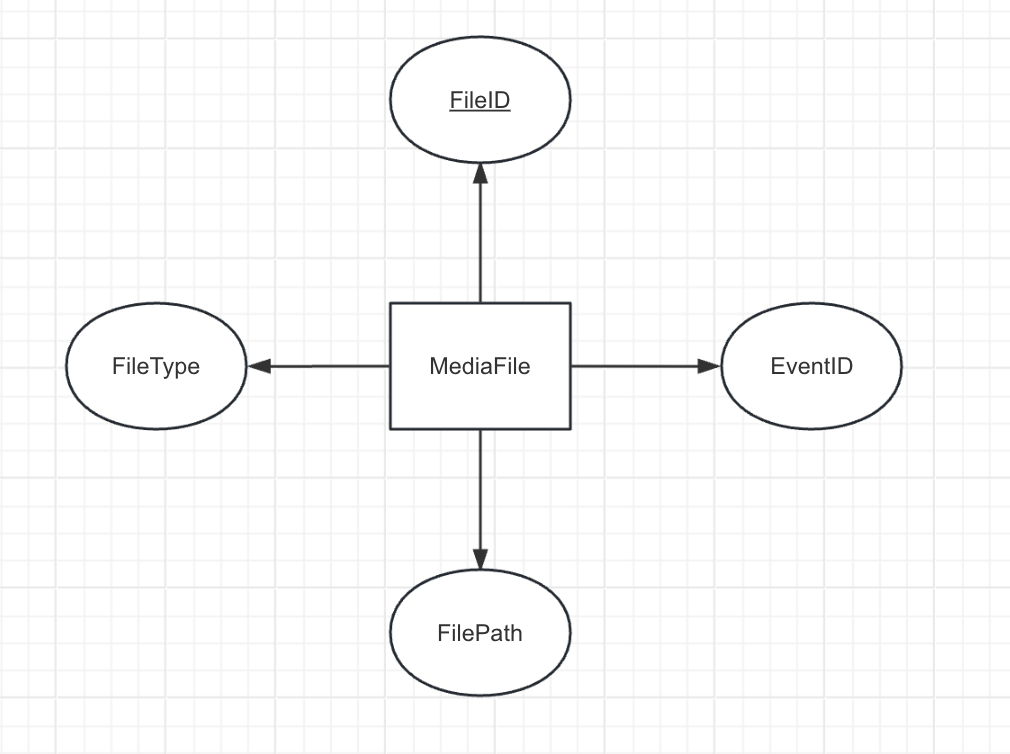
\includegraphics[width=0.5\textwidth]{figures/db-img-03.png}
    \caption{多媒体文件实体图}
    \label{fig:entity-mediafile}
\end{figure}

\subsubsection{通知 (Notification)}

通知实体存储了系统中发送给用户的通知信息,包括通知标识、接收用户ID、内容、发送时间和状态。主键是通知标识,外键是接收用户ID。如\cref{fig:entity-notification}所示,具体介绍如下:

NotifyID:通知标识,主键。每个通知的唯一标识符,用于区分不同的通知。
ReceiverID:接收用户ID,外键,引用用户实体中的UserID。用于标识通知的接收者。
Content:内容,通知的具体内容。用于向用户传达信息。
SendTime:发送时间,通知发送的具体时间。用于记录通知的时间维度。
Status:状态,描述通知的状态,如未读、已读等。用于跟踪通知的处理情况。

\begin{figure}[htbp]
    \centering
    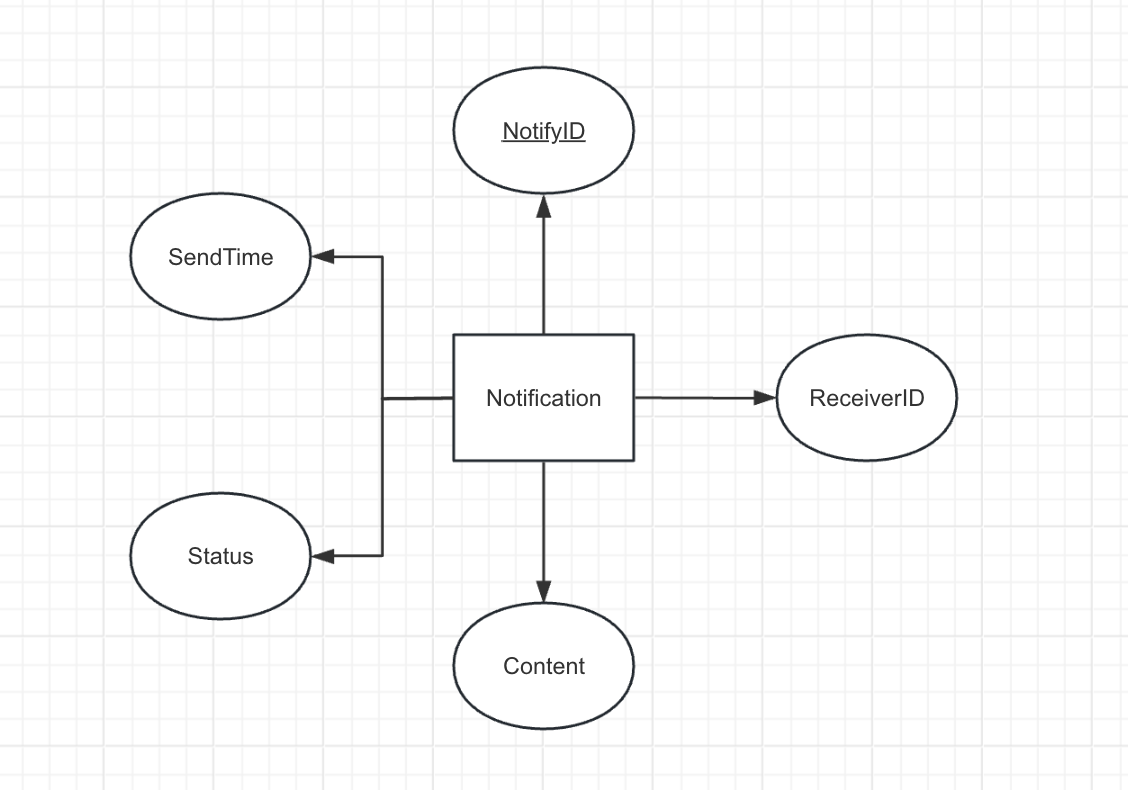
\includegraphics[width=0.5\textwidth]{figures/db-img-04.png}
    \caption{通知实体图}
    \label{fig:entity-notification}
\end{figure}

\subsubsection{用户事件 (UserEvent)}

用户事件实体存储了用户与事件之间的关联信息,包括用户ID和事件ID。复合主键是用户ID和事件ID,分别作为外键引用用户实体和事件实体。如\cref{fig:entity-userevent}所示,具体介绍如下:

UserID:用户ID,外键,引用用户实体中的UserID。用于标识关联的用户。
EventID:事件ID,外键,引用事件实体中的EventID。用于标识关联的事件。

\begin{figure}[htbp]
    \centering
    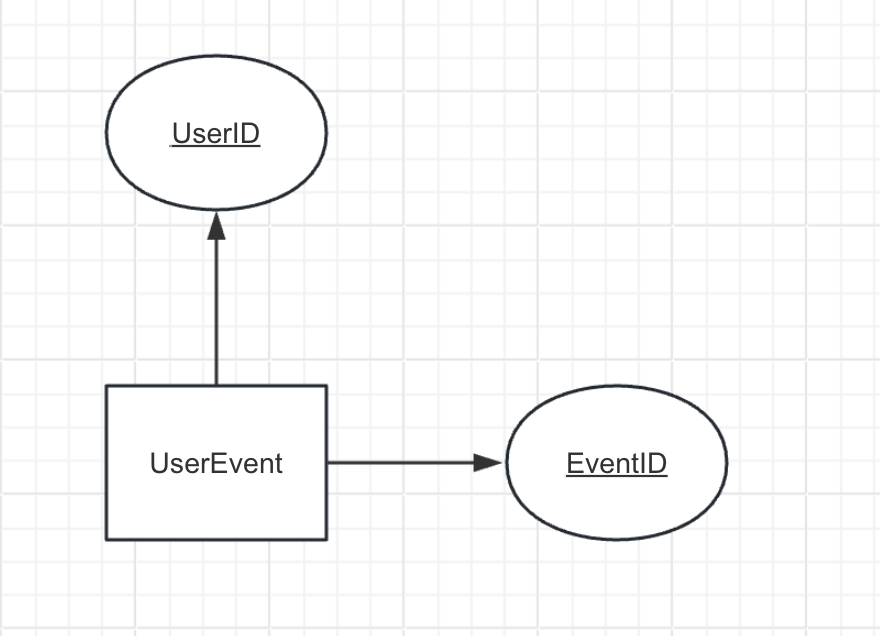
\includegraphics[width=0.5\textwidth]{figures/db-img-05.png}
    \caption{用户事件实体图}
    \label{fig:entity-userevent}
\end{figure}

\subsection{实体联系设计}

\subsubsection{用户与事件之间的联系}

联系类型:多对多

联系描述:一个用户可以上报多个事件,一个事件也可以由多个用户上报(在不同时间或不同地点的同一事件)。为了实现多对多的关系,我们使用一个关联表 UserEvent 来管理用户和事件之间的联系。用户与事件之间的 E-R 图如\cref{fig:rela-user-event}所示。

\begin{figure}[htbp]
    \centering
    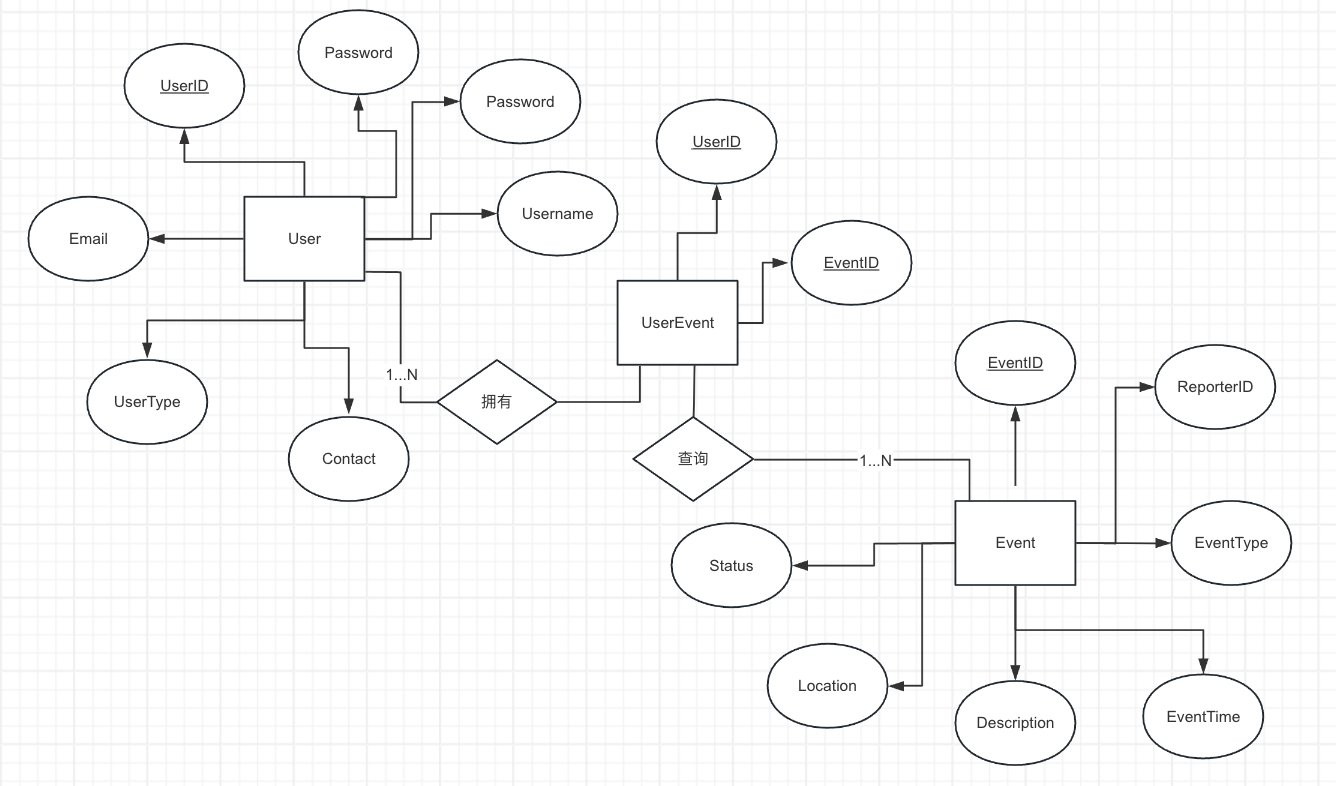
\includegraphics[width=0.5\textwidth]{figures/db-img-rela-01.png}
    \caption{用户事件实体联系图}
    \label{fig:rela-user-event}
\end{figure}

\subsubsection{用户与通知之间的联系}

联系类型:一对多

联系描述:一个用户可以收到多个通知,但每个通知只能发送给一个用户。用户与通知之间的 E-R 图如\cref{fig:rela-user-notification}所示。

\begin{figure}[htbp]
    \centering
    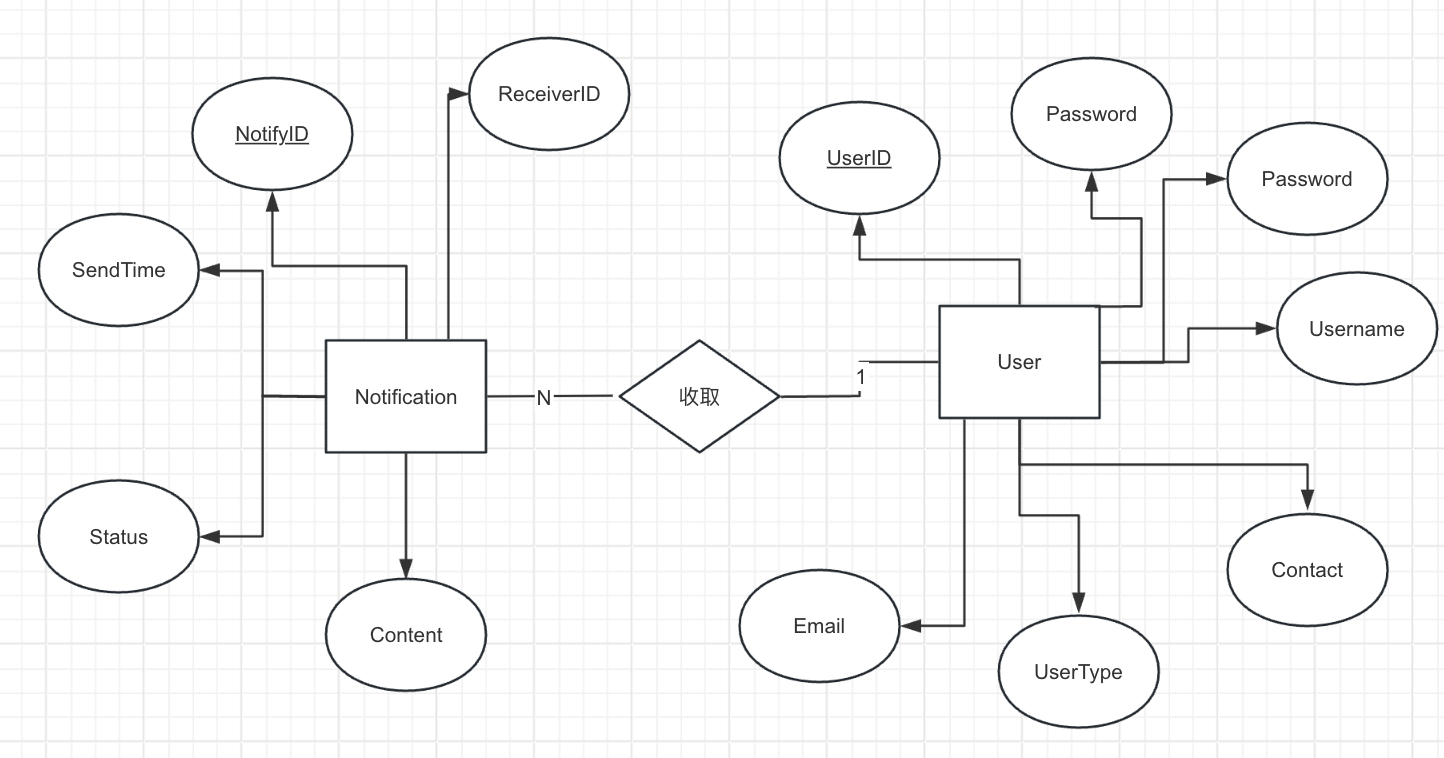
\includegraphics[width=0.5\textwidth]{figures/db-img-rela-02.png}
    \caption{用户通知实体联系图}
    \label{fig:rela-user-notification}
\end{figure}

\subsubsection{事件与多媒体文件之间的联系}

联系类型:一对多

联系描述:一个事件可以关联多个多媒体文件,但每个多媒体文件只能关联一个事件。事件与多媒体文件之间的 E-R 图如\cref{fig:rela-event-mediafile}所示。

\begin{figure}[htbp]
    \centering
    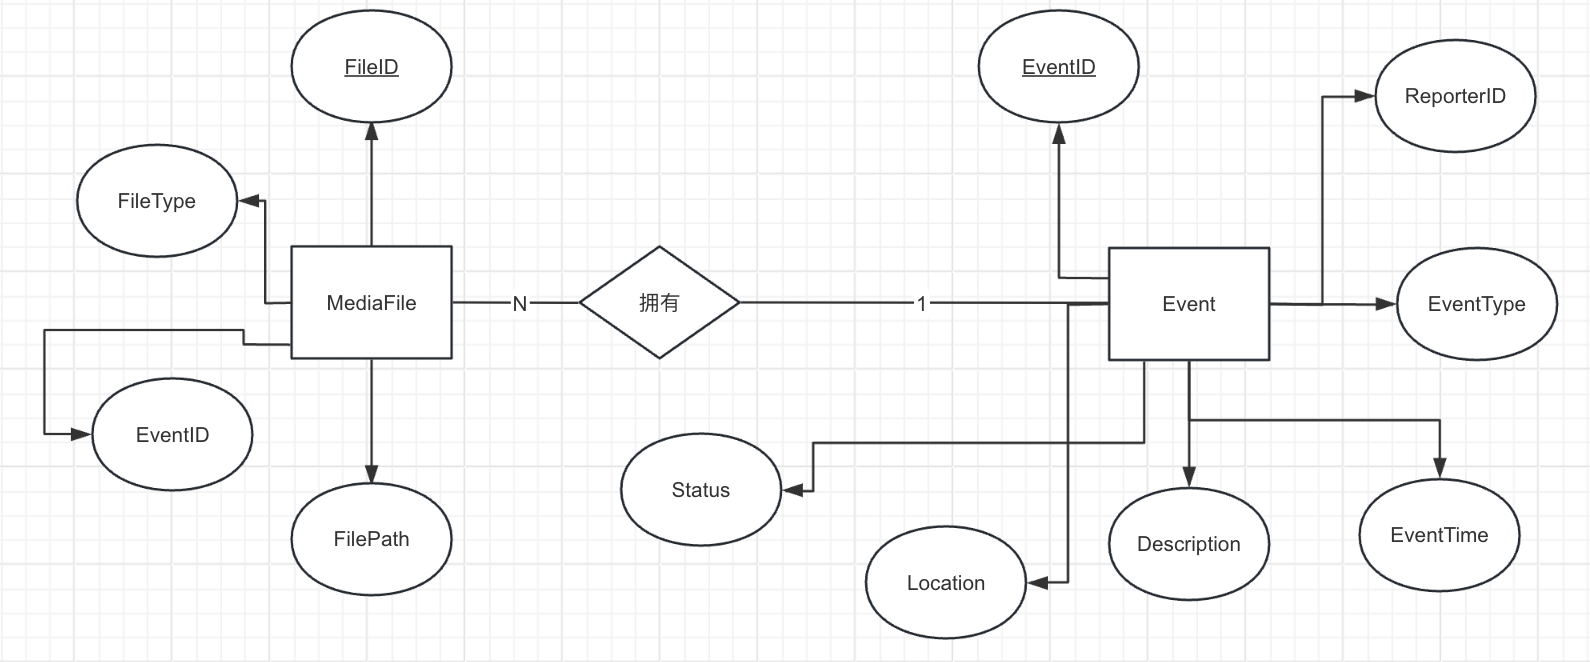
\includegraphics[width=0.5\textwidth]{figures/db-img-rela-03.png}
    \caption{事件多媒体文件实体联系图}
    \label{fig:rela-event-mediafile}
\end{figure}



\subsection{全局E-R图设计}

城市犯罪事件管理平台的全局E-R图,如\cref{fig:rela-tot},描述了系统中各个实体及其相互关系,通过全局E-R图,可以直观地看到系统中各实体之间的关系,确保数据库设计能够有效支持系统的功能需求和业务逻辑。这种设计方式保证了数据的完整性和一致性,同时便于后续的系统开发和维护。

\begin{figure}[htbp]
    \centering
    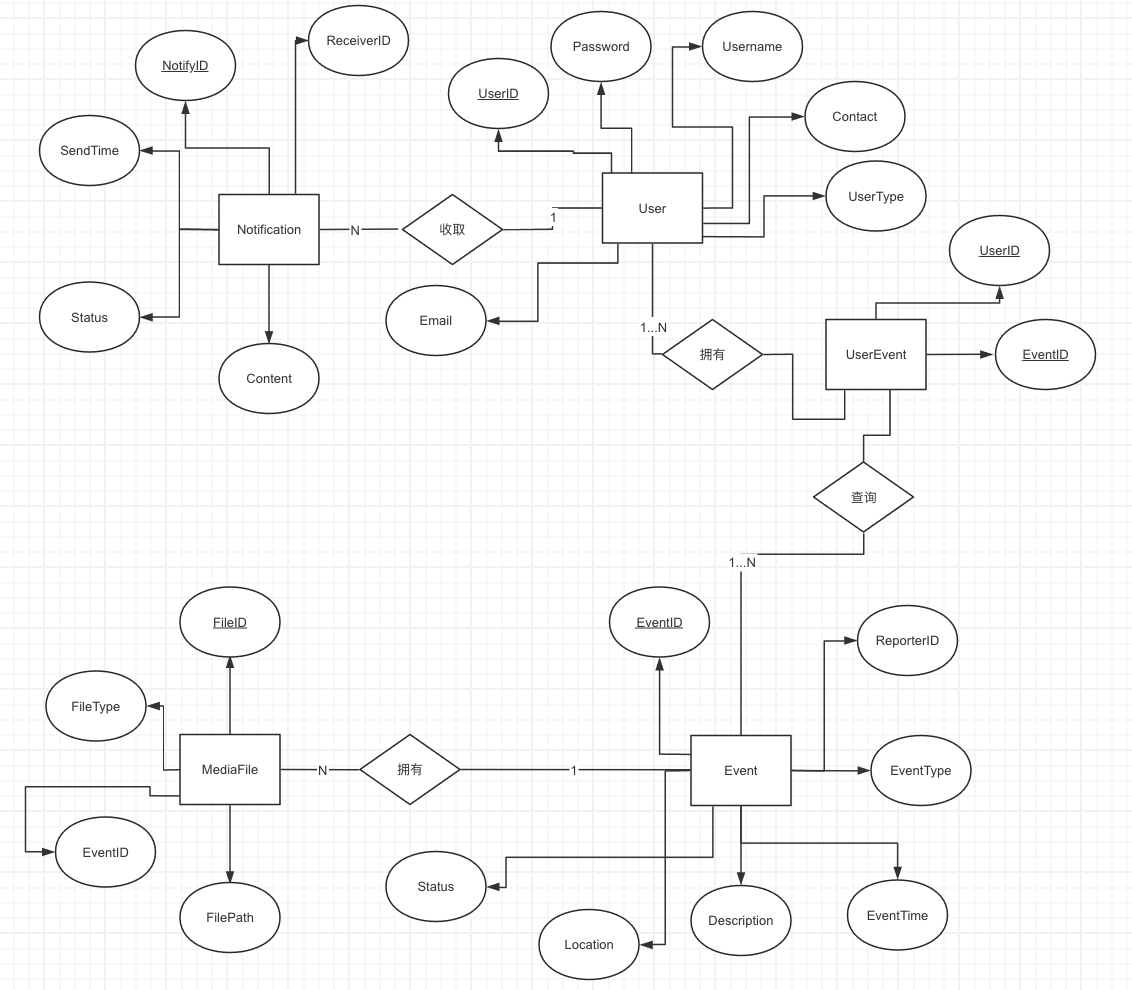
\includegraphics[width=0.5\textwidth]{figures/db-img-rela-tot.png}
    \caption{全局E-R图}
    \label{fig:rela-tot}
\end{figure}
